%%%%%%%%%%%%%%%%%%%%%%%%%%%%%%%%%%%%%%%%%%%%%%%%%%%%%%%%%%%%%%%%%%%%%%%%%%%%%%%
%     enunciado.tex:    Enunciado de la pr�ctica 2 de GIEAI-Inform�tica
%%%%%%%%%%%%%%%%%%%%%%%%%%%%%%%%%%%%%%%%%%%%%%%%%%%%%%%%%%%%%%%%%%%%%%%%%%%%%%%

\documentclass[english,a4paper,11pt]{article}

\usepackage[latin1]{inputenc}  % codificaci�n de caracteres de este archivo
\usepackage[spanish]{babel}    % Traducir: ``abstract'' ---> ``resumen''   etc.
\usepackage{fancyhdr}          % p�ginas con cabecera y pie
\usepackage{listings}          % listados de c�digo fuente
\usepackage{float}             % para que los listados floten como las figuras
\usepackage{vmargin}           % ajuste de m�rgenes f�cil de usar
\usepackage[T1]{fontenc}       % meter fuentes vectoriales
\usepackage{graphicx}          % figuras
\usepackage{upquote}           % comilla recta con \textquotesingle
\usepackage{placeins}          % orden \FloatBarrier para mantener figuras a raya

\usepackage[implicit=false]{hyperref}  % enlaces web (el par�metro implicit=false
                                       % evita problemas con el # de #include etc.)
                                       % uso expl�cito: \href[options]{URL}{text}
                                       %                \url{URL}

% mis abreviaturas
\newcommand{\C}{\texttt{C}}            % escribir� \C en lugar de \texttt{C}
\newcommand{\Pascal}{\texttt{Pascal}}  % idem con \Pascal ...
\newcommand{\fun}[1]{\texttt{#1()}}    % "\fun{main}" ---> "main()" en letra typewriter
\newcommand{\hex}[1]{\texttt{#1}$_{hex}$}
\newcommand{\bin}[1]{\texttt{#1}$_{bin}$}
\newcommand{\enesimo}{\mbox{n-�simo}}
\newcommand{\muvision}{\textit{$\mu\!$Vision4}}
\newcommand{\keilmuvision}{\textit{Keil}~\muvision}
\newcommand{\codigo}[1]{\texttt{#1}}
\newcommand{\menu}[1]{\textit{#1}}

% �rdenes para alternar entre el estilo espa�ol (ligera separaci�n extra
% entre p�rrafos) y el estilo por defecto (p�rrafos junticos junticos)
\newcommand{\parrafosjuntos}{\setlength{\parskip}{0pt}}
\newcommand{\parrafosseparados}{\setlength{\parskip}{1.5ex plus 0.6ex minus 0.5ex}}

% datos importantes del documento
\newcommand{\titulo}{Programming Evolutionary Algorithms with inspyred}     % <<--- T�TULO
\newcommand{\fecha}{}                         % <<--- TEMA
\newcommand{\asignatura}{IASCA}
\newcommand{\institucion}{Departamento de Autom�tica, UAH}
\newcommand{\paginaweb}{http://atc1.aut.uah.es}

% portada
\title{\asignatura \\ \titulo}
\author{\institucion \\ \url{\paginaweb}}
\date{\fecha}

% m�rgenes un poco m�s finos
\setmargrb{25mm}{20mm}{25mm}{20mm}    % left, top, right, bottom

% encabezado y pie
\pagestyle{fancy}
\lhead{\footnotesize \parbox{11cm}{\asignatura}}
\lfoot{\footnotesize \parbox{11cm}{\institucion}}
\cfoot{}
\rhead{\footnotesize \titulo}
\rfoot{\footnotesize P�gina \thepage}
\renewcommand{\headheight}{24pt}
\renewcommand{\footrulewidth}{0.4pt}
%\renewcommand{\headrulewidth}{0pt}

% listados de c�digo fuente flotantes
%\newfloat{floatlisting}{h}{}
%\floatname{floatlisting}{Listado}

% estilo de los listados de c�digo
\lstset{numbers=left,                 % n�meros de l�nea
        numberstyle=\tiny,            % tama�o de los num. de l�nea
        extendedchars=true,           % acentos, e�es...
        %frame=single,                 % marco que encuadra al listado
        basicstyle=\footnotesize\ttfamily,   % tipo de letra
        showstringspaces=false}       % no mostrar espacios de las cadenas

\graphicspath{{figs/}}                % ruta de las figuras

\begin{document} % ------------------ Aqu� empieza el documento ----------------------

% redefinir el nombre de algunas cosas
\renewcommand{\tablename}{Tabla}                  % mejor "Tabla" que "Cuadro"
\renewcommand{\listtablename}{Indice de tablas}
% definidos originalmene en:
%/usr/share/texmf-texlive/tex/generic/babel/spanish.ldf

\maketitle              % montar el t�tulo aqu�� con los par�metros definidos arriba
\thispagestyle{empty}   % no poner n�mero de p�gina ni nada de nada en la 1� p�gina

\renewcommand{\abstractname}{}         % eliminar "Resumen"
\begin{abstract}                       % resumen (sin la palabra "Resumen")
\noindent \textbf{Objectives:}
\begin{itemize}
\item Introduce \texttt{inspyred} programming model
\item EAs solving non-trivial problems
\end{itemize}
\end{abstract}

\sloppy              % hacer m�s flexible el c�lculo del espacio entre palabras para
                     % evitar errores de tipo "overfull box"
                     % (lo contrario de \sloppy es \fussy)

\parrafosseparados   % separaci�n entre p�rrafos (por defecto saldr�n pegados)

\subsection*{Pseudo random numbers generation}
EAs, like any other stochastic search algorithms heavily depends on randomness to solve problems. As a consequence, the algorithm needs to generate a large number of random numbers, which is itself a serious problem. Fortunately, Python's default random number generator works well, and is suitable for using in EC. Given that a computer is a deterministic system, getting randomness from it is complex. For this reason random number are not random, but instead pseudorandom.

In order to properly use a pseudorandom numbers generator we need to feed the algorithm with a seed, i.e., a number that is used to initialize the algorithm. The seed should be as much random as possible, so a common practice is to use the current time, in milliseconds. From an EC perspective, it is important to note that two equal seeds will generate the same pseudoranom number sequence, it means that \textbf{two executions of an EA with the same seed will give the same results}. It is a very important feature, because eases the repetivity of the execution.

For this reason, any well-implemented EA will contain some code to initialize the pseudorandom numbers generator. In the case of  \texttt{inspyred}, you will always find something like

\lstinputlisting{code/pseudo.py}

\subsection*{Getting into inspyred programming API}
Inspyred is a well-documented project. Go to the project website\footnote{\url{http://pythonhosted.org/inspyred/index.html}} and read the following texts:

\begin{itemize}
	\item Read the ``Overview''. Pay special attention to the section ``Design Methodology''
	\item \textbf{Do not} read the tutorial (the following exercises are inspired in those examples)
	\item Examine the examples ``Genetic Algorithm'' and ``Evolution Strategy'' within the ``Examples'' section
	\item Read carefully the subsection ``Customized Algorithms'',  within the ``Examples'' section
\end{itemize}

Once you got a general understanding on the structure of \textit{inspyred}, you should get used to handle its reference manual and source code. Much of the features are not documented, and many times there are doubs that requires reading the source code. Based on the reference library~\footnote{Located in \url{http://pythonhosted.org/inspyred/reference.html}}, answer the following questions.

\begin{enumerate}
	\item Identify all the \textit{mutation} methods available by default.
	\item Identify all the \textit{recombination} methods available by default.
	\item Identify all the \textit{parent selection} methods available by default.
	\item Identify all the�\textit{survivor selection} methods available by default.
	\item Identify all the�\textit{termination} methods available by default.
	\item Identify all the methods available to inspect the population throughout the evolutionary process.
\end{enumerate}


\subsection*{Playing with inspyred}

Based on the code of the one-max problem introduced in the previous practical assigment, perform the following tasks.

\begin{enumerate}
	\item Change the selection method to fitness proportionale.
	\item Change the crossover to uniform crossover.
	\item Change the mutation to scramble mutation.
	\item Show the basics statistics (best, worst and average fitness) for each generation. Use the proper observer.
	\item Store all the individuals in a CSV file for futher analysis. Use the proper observer.
	\item Bonus track: Visualize in real-time the basic fitness statistics in a plot. Use the proper observer.
\end{enumerate}

\subsection*{Genetic operators customization}

We are going to use a variant of the one-max problem. Instead of an all-ones chromosomes, we want to generate a chromosome with the pattern $[0,1,1,1]$ repeated $k$ times, for instance, $[0,1,1,1,0,1,1,1,0,1,1,1]$ with $k=3$. 

Implement a GA to solve the previously described problem. Divide this task into the following steps.

\begin{enumerate}
	\item Implement an skeleton of the algorithm with \textit{inspyred} with default components.
	\item Define and implement the fitness function.
	\item Implement a customized crossover operator that only splits chromosomes in the boundaries of the repeated pattern $[0,1,1,1]$. Compare this operator with one-point crossover.
\end{enumerate}

\subsection*{Trajectory of a spacecraft to the Moon}
\begin{center}
(Based on the problem exposed in the inspyted tutorial, do not read it!)
\end{center}

This exercise deals with an optimization problem of a real-valued function. The objective is to design the trajectory of a spacecraft in orbit on Earth to the Moon using a gravity assist maneuver (see Figure \ref{cap:moon}). For simplicity the problem is reduced to 2D, and there is only one boost at the begining of the journey. With those considerations, the parameters to optimize are:

\begin{center}
\begin{figure}
\centering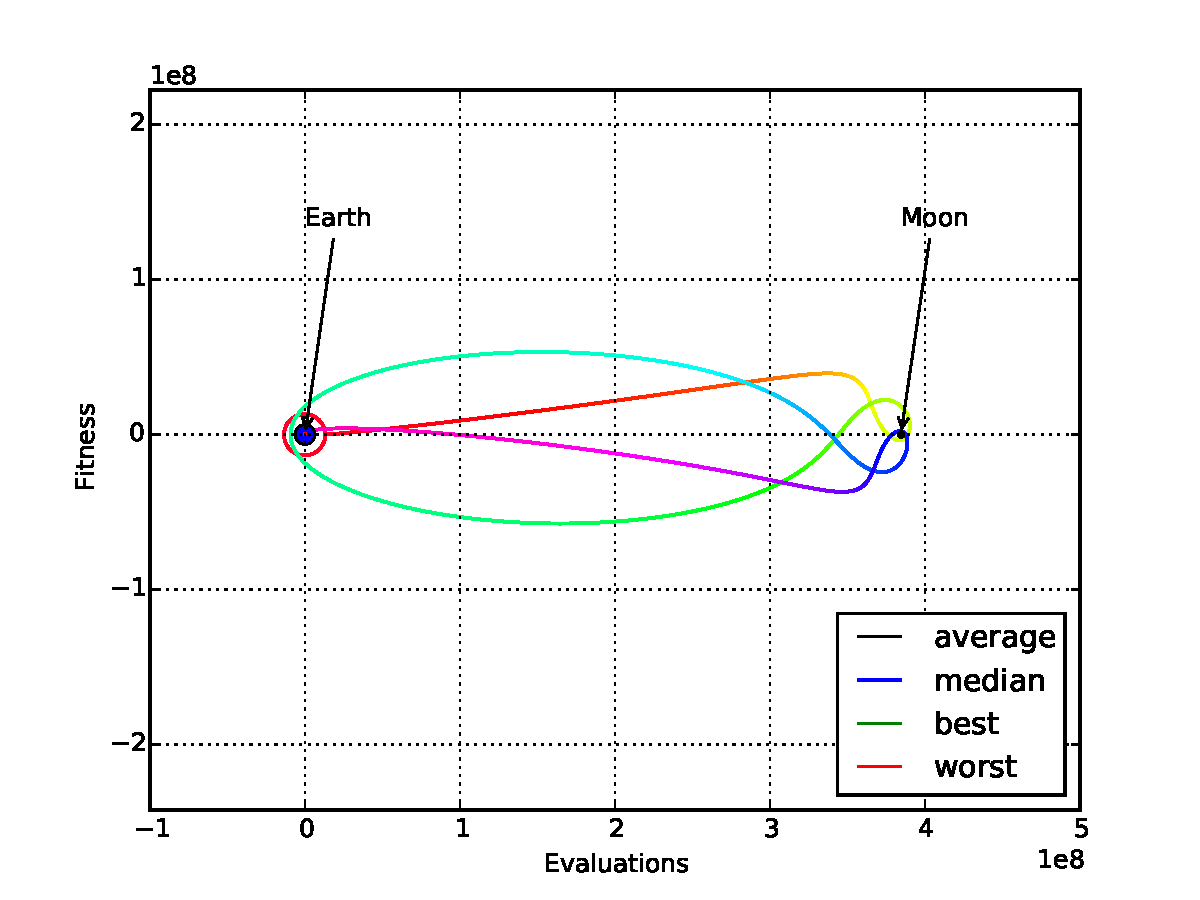
\includegraphics[width=0.6\linewidth]{figs/orbita.pdf}
\caption{Example of evolved trajectory to the Moon and return.\label{cap:moon}}
\end{figure}
\end{center}

\begin{itemize}
	\item \textbf{Orbital height}. The spacescraft begins in a circular orbit over the Earth. This parameter sets its height.
	\item \textbf{Satellite mass}. 
	\item \textbf{Boost velocity}. Velocity after the engine boost. It is a bidimensional vector in form $(x, y)$.
	\item \textbf{Initial y velocity}. Initially, the spacecraft moves in the Y axis with the velocity given by this parameter. It does not move in X.
\end{itemize}

The spacecraft must go to the Moon, transit it as close as possible, and return to land on Earth. It must not crash to the Moon (given by a distance equal to $0$). To this end, we have the following fitness function:

\begin{equation}
f = \frac{d_m}{1000} + d + c - l
\end{equation}

Where $d_m$ is the mimimum distance from Moon, $d$ the total distance traveled, $c$ Moon crash penalty ($1000$) and $l$ Earth landing reward ($1000$). Therefore, this is a minimization problem. Execute the following tasks.

\begin{enumerate}
	\item Download the code that implements the fitness function (\texttt{moonshot}) and test it. The Boost velocity must be given in vectorial form $(x, y)$.
	\item Design and implement an EA that solves the given problem.
	\item Modify the algorithm to consider the following constrains (Hint: Use Bounders)
	\begin{itemize}
		\item Orbital height $\in (6e6, 8e6)$
		\item Satellite mass $\in (10.0, 40.0)$
		\item Boost velocity $(x, y) \in ((3e3, 9e3), (-10000.0, 10000.0))$
		\item Initial y velocity $\in (4000, 6000)$
	\end{itemize}
\end{enumerate}

Once you had finished, compare your solution with the one proposed by the tutorial\footnote{\url{http://pythonhosted.org/inspyred/tutorial.html\#lunar-explorer}}.

\end{document}
